\begin{spacing}{1}
    \chapter*{Abstract}
\end{spacing}
\begin{wrapfigure}{r}{0.3\textwidth}
    \begin{center}
      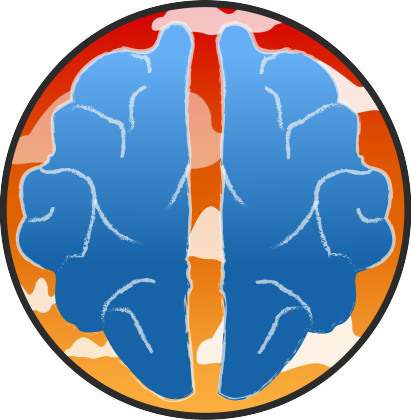
\includegraphics[width=0.2\textwidth]{pics/memoryland-logo.png}
    \end{center}
\end{wrapfigure}

Memories in the form of photos and videos are a valuable part of life, yet they are often 
lost or rarely revisited. To keep these memories alive, an appealing presentation and easy 
accessibility are essential.

The diploma project Memoryland was developed to address exactly this issue. It allows 
personal memories to be experienced in an interactive and animated form. As part of 
this project, a web application was created that transforms photos into engaging 
animations. Users can generate videos from these animations and share them with their friends.

A special focus was placed on creating an immersive experience. Memorylands enable 
users to relive their memories in virtual environments such as a forest or an island. 
Additionally, great care was taken to ensure that the functionalities are as intuitive
and comfortable as possible.

Ultimately, this project aims to make it easier for people to preserve their memories 
in a creative and entertaining way while allowing them to rediscover them effortlessly.

\newpage
\begin{spacing}{1}
    \chapter*{Zusammenfassung}
\end{spacing}
\begin{wrapfigure}{r}{0.3\textwidth}
    \begin{center}
      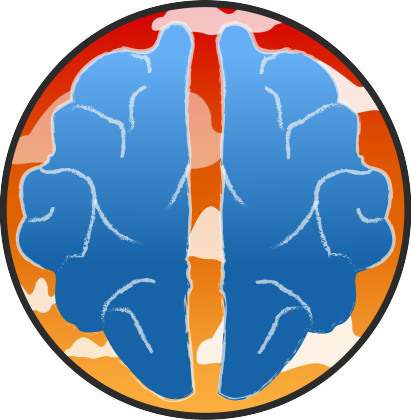
\includegraphics[width=0.2\textwidth]{pics/memoryland-logo.png}
    \end{center}
\end{wrapfigure}
Erinnerungen in Form von Fotos und Videos sind ein wertvoller Bestandteil des Lebens und doch
gehen sie oft verloren oder werden selten angesehen. Um diese Erinnerungen lebendig zu halten,
sind daher eine ansprechende Präsentation und einfache Zugänglichkeit essenziell.

Die Diplomarbeit Memoryland wurde entwickelt, um genau dieses Problem zu lösen. Sie ermöglicht es, 
persönliche Erinnerungen in einer interaktiven und animierten Form zu erleben. Im Rahmen dieser 
Arbeit wurde eine Web-Anwendung erstellt, die Fotos in ansprechende Animationen umwandelt. 
Daraus können Nutzer:innen nun Videos generieren und an ihre Freunde weitergeben.

Besonderes wurde hierbei auf eine immersive Erfahrung geachtet. Memorylands ermöglichen es, 
Erinnerungen in einer virtuellen Umgebung, wie einem Wald oder einer Insel, zu erleben. Es
wurde auch darauf geachtet, dass die Funktionalitäten so intuitiv und gemütlich wie möglich
sind.

Schlussendlich soll unsere Arbeit es Menschen erleichtern, ihre Erinnerungen auf eine 
kreative und unterhaltsame Weise zu wahren und leicht wiederzuentdecken.

